\subsection{Student-Teacher Perceptron}
\label{sxn:SMOG_main-student_teacher}
%\label{sxn:ST-unified-intro}

In this subsection, we present a unified view of the \emph{\StudentTeacher} (ST) \Perceptron 
model from both a practical and a theoretical perspective.  
From the practical (\emph{operational}) side, imagine a real-world practitioner training a large-scale neural network (NN); \cyan{call this NN the \Teacher.
We wish to assess the Teacher’s \emph{true} accuracy on ground-truth labels in consistently reproducing its own (possibly imperfect) outputs. One can then train one or more similar networks -- called \Student(s) -- to mimic the Teacher’s predictions.}
By comparing Student and Teacher outputs, one can approximate the \red{Teacher’s} generalization performance even without an explicit hold-out set.  
Notably, if the Teacher perfectly interpolates its training data, the Student’s error directly estimates the Teacher’s \emph{true} \GeneralizationAccuracy.
Otherwise, it captures the Teacher’s \emph{Precision} in reproducing its own noisy or biased labels.

From the theoretical side, we seek a succinct, analytic formulation of the ST \AverageGeneralizationError, denoted $\AVGSTGE$.  
We work in the \AnnealedApproximation (AA) -- a simplification often valid when networks are sufficiently large and can nearly interpolate their training data. 
Under this approximation, one obtains closed-form expressions for the \StudentTeacher \emph{Overlap} $(R)$
and thus for the \Teacher’s overall error or accuracy.  
These results lay the foundation for our \emph{\SemiEmpirical} approach, in which we supplement this theoretical form with empirical measurements (e.g., from the trained weight matrices) to account for real-world correlations in the data and the model’s internal structure.  

\cyan{I\textbf{Take note that we deviate from the standard \SMOG ST model in an important way} -- we make no direct assumption that the labels are realizable by a \Teacher NN. \SETOL makes its realizability assumption in a novel way: rather than assume that there exists an unknown \Teacher that \emph{generates} the labels $\Yt$ implicitly
This point is both subtle -- since the derivations will proceed almost identically to those found in~\cite{engel2001statistical,EngelAndVanDenBroeck,SST90,SST92}
-- and also radical, because our derived  quality metrics $\Q$ now
depend directly on empirical measurables of the \Teacher.
\textbf{As far as we know, this is completely new.}
}

\begin{enumerate}[label=4.3.\arabic*]
\item
  \textbf{Operational Setup.}
  In subsection~\ref{sxn:ST_OP_setup} we explain how to set up the \cyan{our formulation} \StudentTeacher
  model in an \emph{operational} manner. 
  In particular, we emphasize the difference between \emph{true accuracy} (vs.\ ground-truth labels)
  and \Precision (vs. the Teacher’s own labels). We also the discuss the difference between
  our \Quality metrics and the \emph{Generalization Gap}.

  \item
    \textbf{Theoretical Student-Teacher Average Generalization Error $(\AVGSTGE)$.}
    In subsection~\ref{sxn:SMOG_main-st_av}  we outline how to derive $\AVGSTGE$ using the AA.  
    We introduce the key expressions that will serve as the starting point for our extended \SemiEmpirical theory in Section \ref{sxn:matgen}.
\end{enumerate}

\subsubsection{Operational Setup}
\label{sxn:ST_OP_setup}
\begin{figure}
%  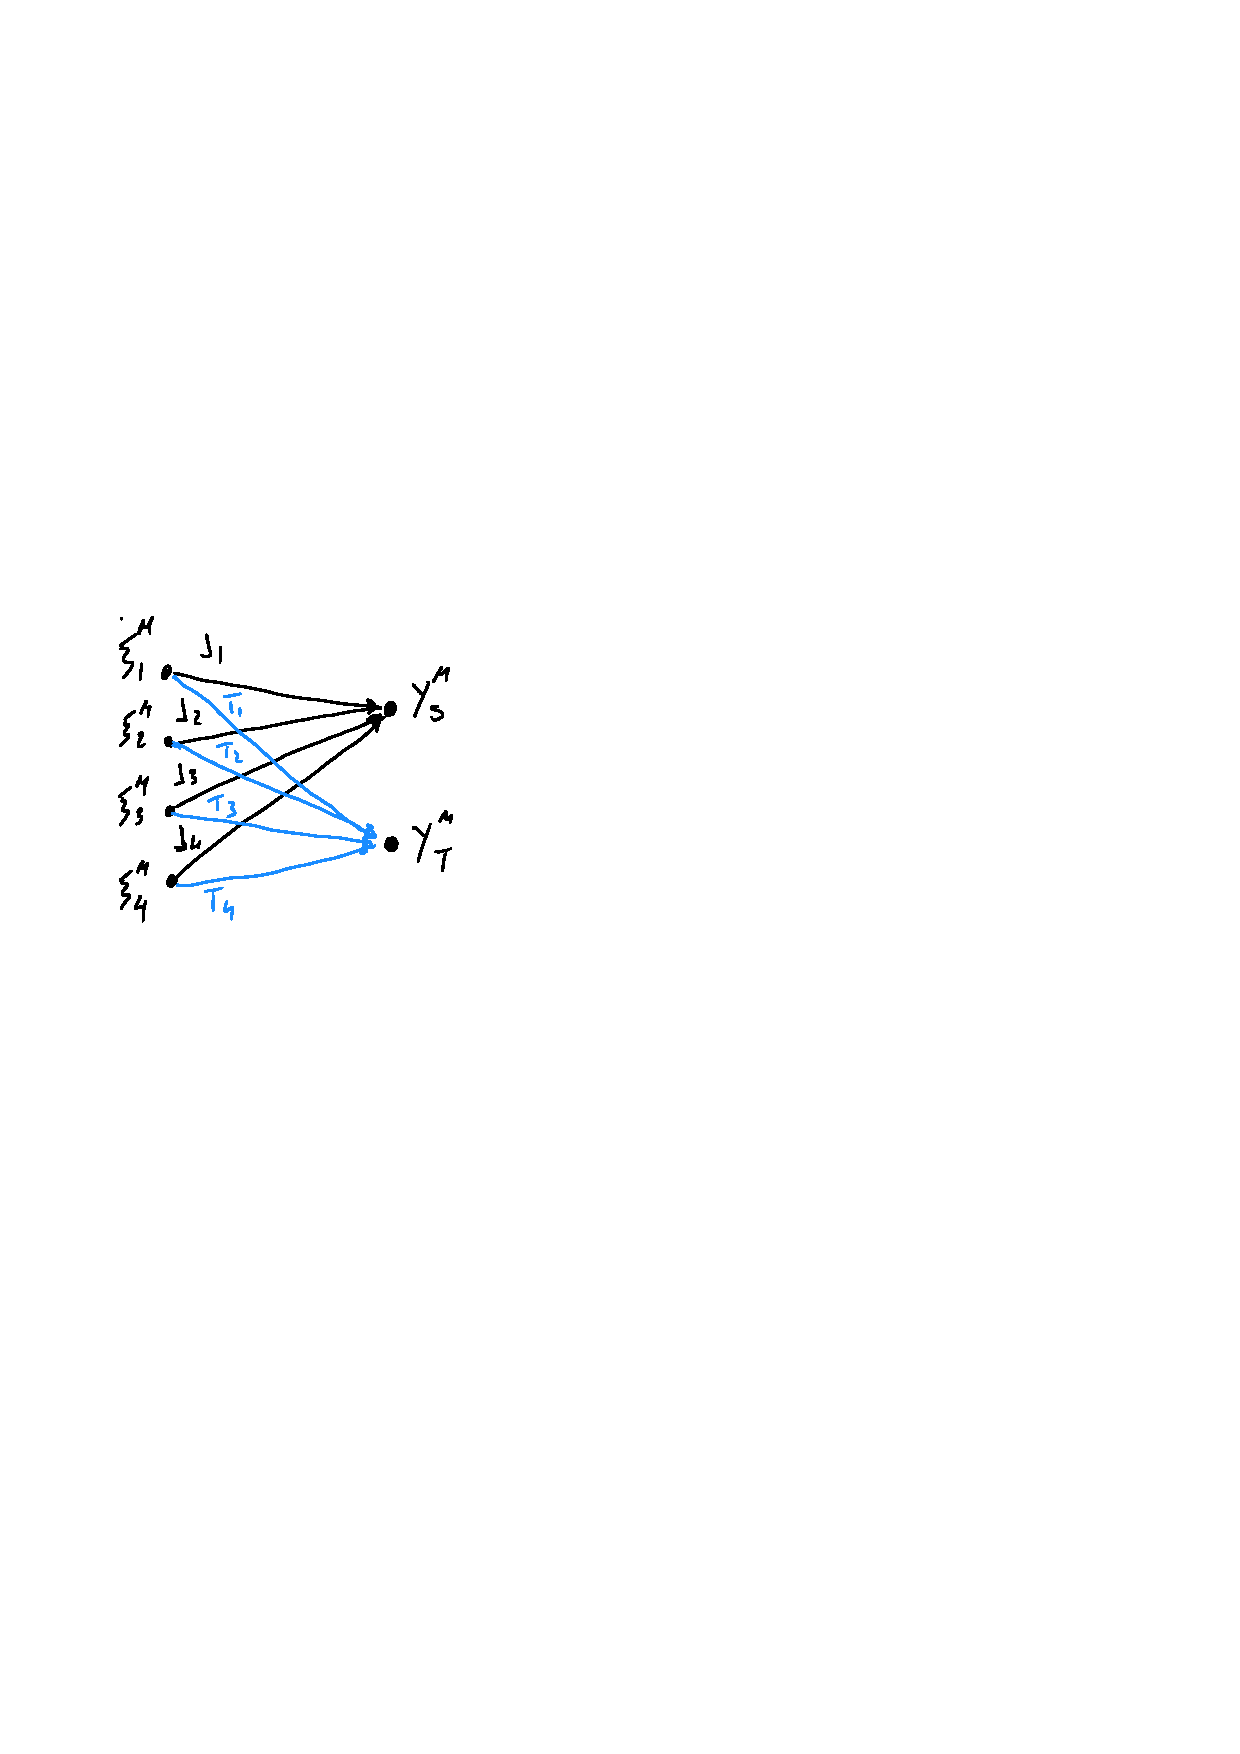
\includegraphics[width = 0.3\textwidth]{./img/perceptron.pdf}
  \begin{center}
    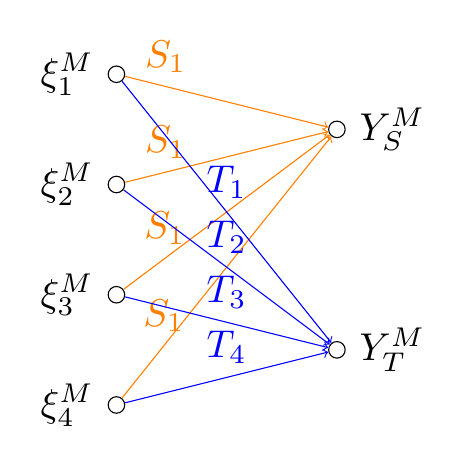
\begin{tikzpicture}[scale=1.4, every node/.style={transform shape}]
    \node[draw, circle, minimum size=0.15cm, inner sep=0.05cm] (A) at (0, 3) {};
    \node[draw, circle, minimum size=0.15cm, inner sep=0.05cm] (B) at (0, 2) {};
    \node[draw, circle, minimum size=0.15cm, inner sep=0.05cm] (C) at (0, 1) {};
    \node[draw, circle, minimum size=0.15cm, inner sep=0.05cm] (D) at (0, 0) {};

    \node[left] at (A.west) {$\xi_1^M$};
    \node[left] at (B.west) {$\xi_2^M$};
    \node[left] at (C.west) {$\xi_3^M$};
    \node[left] at (D.west) {$\xi_4^M$};

    \node[draw, circle, minimum size=0.15cm, inner sep=0.05cm] (Y) at (2, 2.5) {};
    \node[draw, circle, minimum size=0.15cm, inner sep=0.05cm] (Z) at (2, 0.5) {};

    \node[right] at (Y.east) {$Y_S^M$};
    \node[right] at (Z.east) {$Y_T^M$};
  
    % Arrows
    \draw[->, orange] (A) -- (Y) node[pos=0.2, above] {$S_1$};
    \draw[->, orange] (B) -- (Y) node[pos=0.2, above] {$S_1$};
    \draw[->, orange] (C) -- (Y) node[pos=0.2, above] {$S_1$};
    \draw[->, orange] (D) -- (Y) node[pos=0.2, above] {$S_1$};

    \draw[->, blue] (A) -- (Z) node[pos=0.5, above] {$T_1$};
    \draw[->, blue] (B) -- (Z) node[pos=0.5, above] {$T_2$};
    \draw[->, blue] (C) -- (Z) node[pos=0.5, above] {$T_3$};
    \draw[->, blue] (D) -- (Z) node[pos=0.5, above] {$T_4$};

  \end{tikzpicture}
  \end{center}
  \caption{Pictorial representation Student and Teacher Perceptrons.}
\end{figure}



Here, describe the basic setup of the classic \StudentTeacher model, taking an operational view from the perspective of a practitioner training real-world \Student and \Teacher models.  Specifically, we present the \AnnealedApproximation (AA) in a practical light,
and use it explain the difference between computing the \emph{Empirical\GeneralizationError}, $\AVGEMPGE$, for the \emph{\TrueAccuracy}
and for the \emph{\Precision} of a \Teacher model.

\paragraph{Test Error of the Teacher}

We start by describing how to obtain a simple formal expression for the empirical test errors of the \Teacher, first for the \TrueAccuracy.

Let us say we have a model, called \Teacher $(T)$, which maps some \emph{actual} (i.e., correlated) data
$\DATA\in\ADD$ to some known or \emph{true}  labels $(\Ytrue)$
(where,  $\Ytrue$ is, say, an $N$-dimensional vector of binary labels).
We might say that $\Ytrue$ represents the \emph{\GroundTruth} for the problem.
Operationally, we train the \Teacher $T$ to reproduce or at least approximate the true labels $\Ytrue$.
\begin{align}
 T:\DATA\rightarrow \Yt \approx \Ytrue.
\end{align}
If $T$ reproduces the true labels exactly, we might say that the \Teacher has been
trained to \emph{\Interpolation}, and, therefore, $\Yt = \Ytrue$.
Indeed, most models today are trained to \emph{\Interpolation}, and we don't need to
necessarily worry about the difference between the true and the predicted \Teacher labels.
Formally, however, and to understand better the \AA, it is beneficial to discuss the implication
of this distinction.

Following \EQN~\ref{eqn:dnn_energy}, lets say the \Teacher outputs are specified
by an  Energy function $E^{T}_{NN}$
\begin{align}
\label{eqn:T_ENN}
\Yt=E_{NN}(T,\DATA) 
\end{align}
\footnote{Do not confuse the Energy/output function $E_{NN}$ with the energies $\mathbf{\Delta E}$  defined below to represent the ST error function(s).  We refer to outputs of $E_{NN}(\TVEC,\DATA )$, when applied to a data point $\DATA$, as energies because they are effectively un-normalized probabilities for the class outputs (for labels $\Ymu=1$ or $-1$).  }
so that we may write the \emph{Empirical} \AverageTrainingError
$\AVGEMPTE$
as 
\begin{align}
\label{eqn:Eg_train}
\AVGEMPTE:= \frac{1}{N^{train}}\sum_{\mu=1}^{N^{train}}\mathcal{L}[\Ytrain,E_{NN}(T,\DATAtrain)]  .
\end{align}
Ideally, we seek the \emph{True} \AverageGeneralizationError of the \Teacher, denoted  $\AVGGE^{T}$. 
Of course, this is unknowable, but in practice, we estimate $\AVGGE^{T}$ 
by measuring the error of the \Teacher predictions on some test (or hold-out) set $(\DATA^{test}, \MY^{test})$.
We call this the \emph{Empirical \AverageGeneralizationError}, $\AVGEMPGE$, and write
\begin{align}
\label{eqn:Eg_test}
 \AVGGE^{T}\approx \AVGEMPGE:= \frac{1}{\Ntest}\sum_{\mu=1}^{\Ntest}\mathcal{L}[\Ytest,E_{NN}(T,\DATAtest)] .
\end{align}
To measure the error, the loss function $\mathcal{L}$ may be a L1 $(\ell_1)$ or L2 $(\ell_2)$ loss;
whereas for training a model, it is usually something like a cross-entropy loss, but this detail does matter later.

If we don't have a hold-out set, however, we can still estimate $\AVGGE^{T}$ using the \Student-\Teacher approach.

\paragraph{Estimating the Teacher Error with Students: Accuracy vs. Precision}

Imagine training a \Student $(S)$  model (with a similar architecture as $T$, and acting on the same  
dataset $\DATA\in\ADD$), which tries to  reproduce the \Teacher predictions:
\begin{align}
S:\DATA\rightarrow \Ys \approx \Yt  ,
\end{align}
and assume the \Student outputs $\Ys$ are given by the Energy output function $E^{S}_{NN}$
\begin{align}
\label{eqn:S_ENN}
\Ys=E_{NN}(S,\DATA) ,
\end{align}

\begin{figure}[ht] % [h] places the figure approximately here
  \centering
  \resizebox{0.75\textwidth}{!}{

\begin{tikzpicture}

    % Axis
%    \draw[->] (0,0) -- (0,4) node[left] {Predictions};
    \draw[->] (0,0) -- (6,0) node[below] {Value};
    
    % Gaussian distribution
    \draw[thick, red] plot [smooth] coordinates {(1,0) (2,1) (3,3) (4,1) (5,0)};
    
    % Ground Truth line
    \draw[thick, blue] (3,0) -- (3,3.2);
    \node[blue, above] at (2.5,3.2) {\textbf{Accuracy} };
    \draw[->] (2.5,3.) -- (3,3.);
    \node[black, below] at (0.75,3.2) {\textbf{Teacher output} $\Yt$};

    % Accuracy bracket
    \draw[<->, blue, thick] (3,3.2) -- (4,3.2);
    
    % Teacher (high accuracy, low precision)
    \fill[darkgreen] (4,3) circle (0.15);
    \node[right, below] at (5.5,2.9) {\textbf{Ground truth} $\Ytrue$};
    
    % Student outputs (spread)
    \draw[->] (2.5,1) -- (3.5,2);
    \node at (0.75,0.75) {\textbf{Student outputs} $\Ys$};

    % Precision label
    \draw[<->, red, thick] (1,-0.5) -- (5,-0.5);
    \node[red, below] at (3,-0.5) {\textbf{Precision}};
    
    % Bullseye diagram (Right side)
    \begin{scope}[xshift=9cm, yshift=2cm]
        \draw[thick] (0,0) circle (1.8);
        \draw[thick, fill=white] (0,0) circle (1.2);
        \draw[thick, fill=white] (0,0) circle (0.6);

        \fill[blue] (-0.5, 0.0) circle (0.10);
        % Random student outputs
        \foreach \x/\y in {-0.6/0.3, 0.1/-0.7, -0.15/0.5, -0.3/-0.5, -0.75/0.75, -0.9/-0.2} {
            \fill[red] (\x,\y) circle (0.08);
        }
        
        % Teacher dot in center
        \fill[darkgreen] (0,0) circle (0.15);
        
        \node[left] at (2.,-2.5) {\textbf{Bullseye Example}};
    \end{scope}

\end{tikzpicture}
  }
  
\caption{Precision vs. Accuracy}
 \label{fig:precision}
\end{figure}

If the \Teacher is trained to \Interpolation, then the difference between
the \Student and the \Teacher labels 
estimates the true error, i.e., $\Vert\Ys-\Yt\Vert=\Vert\Ys-\Ytrue\Vert$,
and this error is associated with the \TrainingAccuracy of the model in predicting the \GroundTruth.
But if the \Teacher makes some errors, then $\Vert\Ys-\Yt\Vert$
is now estimating the \Precision of the model.
These two situations are depicted in Figure~\ref{fig:precision}.

The \StudentTeacher model also explains why NNs can generalize even even when trained to \Interpolation on noisy data (which has been a source of confusion \cite{Understanding16_TR}).  In this model, the \GeneralizationError  $\AVGGE^{T}$ is a simple function of the overlap $R$ between the \Teacher $T$ and the \Students $S$, i.e., $\AVGGE^{T}\sim \THRMAVG{1-\EPSLR}$.  So even if the \Teacher $T$ is trained on noisy data, as long as there are \Students $S$ with significant overlap $R$ with the \Teacher, the \Teacher \GeneralizationError  $\AVGGE^{T}$  can be considerably small.  For more details, see \cite{MM17_TR_v1}


\paragraph{Learning the Student}
Moving forward, we will always assume the \Teacher is trained to \Interpolation because this
actually corresponds to the \AnnealedApproximation, whereas if the \Teacher makes
errors, we may need to consided  \Quenched averages, explained below.

Imagine now that in order to estimate the empirical \AverageGeneralizationError, $\AVGEMPGE$,
by training a very large number of Students, and computing the average ST error on some test set.
Let us break the data set into training $\DATAtrain$ and test $\DATAtest$ examples, 
train models on the training data (that is, find the optimal model weights), 
and evaluate the $S$ and $T$ models on the test data.

The \Student learning task can be written as in \EQN~(\ref{eqn:dnn_opt})
as the following optimization problem over the training data:
\begin{align}
\underset{\{S'\}}{\argmin}\sum_{\mu=1}^{N^{train}}\mathcal{L}[E_{NN}(S',\DATAtrain),E_{NN}(T,\DATAtrain)]   ,
\label{eqn:ST-learning-task}
\end{align}
%Notice that, at this step, the \Student $S$ and the \Teacher $T$ both depend explicitly on the specific choice of the training data $\DX_{train}$.  
%That is, we could write $S[\DX^{train}], T[\DX^{train}]$.

If the \Teacher is trained to \Interpolation, then the optimization problem in \EQN~\ref{eqn:ST-task} is
training a \Student to reproduce the \GroundTruth labels, so that $\Ys\sim y_{\mu}^{true}$
for both the training and test sets.
\begin{align}
\underset{\{S'\}}{\argmin}\sum_{\mu=1}^{N^{train}}\mathcal{L}[E_{NN}(S',\DATAtrain),\Ytrue]   ,
\label{eqn:ST-learning-intepolation}
\end{align}

But if not, then the \Student is reproducing the possibly
incorrect \Teacher labels, and, importantly, the \Student $S$ now depends explicitly
on how the \Teacher was trained.  That is, we should denote that the learned
\Student explicitly depending on $T$, i.e. $S\rightarrow S[T]$.
This will be important below.

\paragraph{The \AverageGeneralizationError}
In either case, however, we may still estimate the Empirical \AverageGeneralizationError
by replacing the test predictions in \EQN~\ref{eqn:Eg_test} with the student predictions
$y_{\mu}^{test}\rightarrow \Ys$, and then averaging directly over the test data $\DATAtest$
for all possible or available test examples.

If we have a very large number of suitable Students
(say, drawn from some random distribution), then we can try to estimate the 
\AverageGeneralizationError of the \Teacher, i.e., $\TGE^{T}\approx\AVGEMPGE$.
$\AVGEMPGE$ is given by an average loss, the average is 
over all possible Students $N_S$,  and then  over all  $\Ntest$ test data points $\DATAtest\in\mathbf{D}$ 
\begin{align}
  \AVGEMPGE
  &=
  \frac{1}{\Ntest}\sum_{\mu=1}^{\Ntest}
  \frac{1}{N_S}\sum_{S}
  \mathcal{L}[E_{NN}(S,\DATAtest),E_{NN}(T,\DATAtest)]  \\ \nonumber
    &=
  \frac{1}{N_S}\sum_{S}
    \frac{1}{\Ntest}\sum_{\mu=1}^{\Ntest}
    \mathcal{L}[E_{NN}(S,\DATAtest),E_{NN}(T,\DATAtest)] ,
\label{eqn:emp_gen_error}
\end{align}
where (ideally) $\Ntest$ is extremely large.

In Bra-Ket notation, we may also write
\begin{align}
  \AVGEMPGE
  &= \langle \langle \DETOPSTx \rangle_{S} \rangle_{\DXtest}\\ \nonumber
  &= \langle \langle \DETOPSTx \rangle_{\DXtest} \rangle_{S}
\end{align}
where $\DETOPSTx:=\mathcal{L}[E_{NN}(S,\DATAtest),E_{NN}(T,\DATAtest)]$.
For the empirical estimate, it does not matter what order we take the sums in,
but we are not estimating the
the True \AverageGeneralizationError  of the \Teacher, $\AVGGE^{T}$,
unless $T$ is trained to \Interpolation.
For the theoretical estimate, however, the order can be important, and this also depends on
if $T$ is trained to \Interpolation or not.
\footnote{This approach can be likened to the Bootstrap method~\cite{efron1993bootstrap} used for error estimation.  However, the Bootstrap method predominantly emphasizes variations in the input data $\NDX\in\mathbf{D}$, while in this context, we are essentially bootstrapping over the students $S$.}

%\michael{Is this for the optimal values of the parameters in the learning task \EQN~(\ref{eqn:student-learning-task})%?  Presumably not, since we are averaging? }
%\charles{Good question. We do not specify how the hyperparameters are selected.}

\paragraph{Annealed vs. Quenched Averages}
\nred{THIS NEEDS CLEANED UP}
Recall that in the \STATMECH approach to computing errors, we do not break the data into
training and test, but, instead, to obtain the \AverageGeneralizationError, $\AVGGE$, use
the \GeneratingFunction approach. In doing this, we need to compute both the \ThermalAverage
over the model weights ($S,T$), and also take the data average over the entire available model data set $\MDD$
And the order can matter.

In the case where the \Teacher is trained to \Interpolation, may may train the \Student 
independently of \emph{when} the \Teacher.  
But if \Teacher is \emph{not} trained to \Interpolation, then formally we must train the \Teacher
first to obtain target predictions for the \Student.  That is, the \Student formally
depends on the \Teacher, $S[T]$.
The empirical errors in $T$ would then formally depend on the specific instantiation of the data  $\NDXIn\in\MDD$,
and therefore, conceptually imagine that we must first average over the data
before averaging over the weights.
Training to \Interpolation correpsonds conceptually to working with a model
in the \AnnealedApproximation, whereas not correpsonds to \Quenched case.

Practically, when the \Teacher is not trained to \Interpolation, 
we may need to resample the training data and training an ensemble of models to compensate for anomalies in training data (bad labels, noise, etc.) that may cause the underlying model to overfit to the training data.
Theoretically, within \SMOG, this is equivalent to \emph{quenching} the system to the data (a term analogous to quickly cooling a physical system, frezing in any defects).
In contrast, when one \emph{anneals} a physical system, one heats up and cools it down slowly, and repeatedly, thereby removing any defects (of data anomalies for NNs, or material defects in a physical system).

In \STATMECH, one can perform a so-called quenched average using a replica calculation,
effectively removing the dependence on test and/or training data
from the final estimate for $\AVGEMPGE$.
However, the theoretical quenched result may differ significantly from the annealed case when the underlying model is unrealizable~\cite{SST92}. 
This may occur when the training data is very noisy and/or the model architecture is such that it can not correctly predict all the training labels.
In such cases, the model will always have some finite, non-zero Average \TrainingError, $\AVGTE > 0$,
even in the large-$N$ limit of infinite data.  In such a case, this indicates
a highly complex error landscape with many local minima separated by extremely high barriers,
and a slowing down of the dynamics.%
\footnote{In modern ML parlance, one might say the model can not be evaluated at interpolation, although 
in practice such a model might have a zero empirical \TrainingError since it may overfit the specific training data.}
\michael{This seems like important discussion, but it is related to what is going on in Section~\ref{sxn:SMOG_main-spin_glass}; I feel like we should have a minimalistic discussion of things like spin glasses in the main text, and then have a self-contained appendix that goes into it in more detail, since it gets in the way of getting to Section~\ref{sxn:SMOG_main-st_av} and Section~\ref{sxn:matgen}.  }
\charles{This is a minimal discussion.  }

While it is commonplace to train ensembles and/or use cross-validation when training small models (as the above discussion assumes),
this could be extremely expensive and impractical in modern ML, e.g., for very large models like LLMs~\cite{LLMS}.
For such massive NNs, one needs a theory that can detect anomalies in training directly from observations during and/or after training.
This is a hallmark of the \SETOL approach, and it distinguishes \SETOL from the classic \STATMECH approach.
\michael{MM TO DO: Probably move that to the intro.  That is an important par, too imp to be buried here.}
\charles{Not sure.  Intro is already long.  Maybe the conclusions}

%That said, it may be beneficial in practice to use subsamples of the training data to train the \Teacher and the Students
%when, say, the training data has mislabeled and/or noisy data.  With such bad data, the 
%results could be quite different after taking this additional step.
%Indeed, it is exactly these cases where the results differ theoretically as well as in practice.
%We will take a deeper look at such case of noisy data below.

%Importantly, we will not used the quenched form of $\mathcal{E}_{t}^{emp}$ because we will be able todetect
%anomalies in the training data directly by looking at the fitted \SemiEmpirical HT parameter $\alpha$.

be used to estimate the \AverageGeneralizationAccuracy (and not the \Precision),
and which we will refer to more generally as a layer and/or model \Quality.


\paragraph{Generalization Gap vs. Model Quality}
\label{sxn:SMOG_main-model_quality}

We should distinguish between what is typically done in the \SLT literature versus the \STATMECH approaches.
In \SLT, one is typically interested in modeling the \emph{\GeneralizationGap}.
The \GeneralizationGap quantifies the difference between a models performance on training data versus unseen test data:
\begin{align}
  \label{eqn:gen_gap}
  \mathcal{E}^{emp}_{gap}:= \TTE[\DXtrain]- \TGE[\DXtest]
\end{align}
In contrast, in \STATMECH approaches, one considers the \ModelGeneralizationError directly,
which is sometimes called the \ModelQuality in the \SLT literature.
\michael{I think SST looks at generalization error also.  I think this dichotomy isn't quite correct, and it convovles several issues.  It seems most connected with the par around \EQN~\ref{eqn:Qdef} and \EQN~\ref{eqn:GammaQdef}. Maybe we should combine this with that and put is somewhere, removing the incorrect claim/suggestion, and highlighting the ideas in the next par, which are key.
}
\charles{Thats not what this is about.  This is an important section that belongs here.
needs some work}
Model quality is an indication of the models accuracy, precision, recall, or any other relevant metric based on the task at hand.
%Here, we mean that the \ModelGeneralizationError is a measure of the \ModelQuality on such OOD data.

While related, in developing an analytic theory, the \GeneralizationGap and
the \ModelQuality (or \ModelGeneralizationError) require conceptually different approaches.
This is because the  \GeneralizationGap depends on a specific realization of the training data,
whereas our \ModelGeneralizationError will be formulated on a random training data set
(and then corrected later with empirical data).
In this sense, any theory of the \GeneralizationGap  requires a formalism where the
predicted model error is \Quenched to the training data, which is not what we want.
In contrast, the \ModelGeneralizationError  will be formulated using the \AnnealedApproximation (AA),
and is therefore both conceptually and mathematically simpler.
\michael{These ideas seem key; they should either be combined with the par around \EQN~\ref{eqn:Qdef} and \EQN~\ref{eqn:GammaQdef}, or they should be in the intro.}

\nred{Comment on our paper with YQ}




\subsubsection{Theoretical Student-Teacher Average Generalization Error}
\label{sxn:SMOG_main-st_av}

Here, we seek a simple, formal expression for the
\StudentTeacher Average \GeneralizationError, $\AVGSTGE$,
that can be used as the starting point for our extended \SemiEmpirical theory.

%
\begin{figure}[t] %[h] % [h] places the figure approximately here
    \centering
\resizebox{0.75\textwidth}{!}{
\begin{tikzpicture}[
     thick, % Line thickness
    rectnode/.style={rectangle, draw=black, thick, minimum width=6cm, minimum height=2.5cm, rounded corners=0.3cm}, % Rectangular node style with rounded corners
    -> % Arrow style
]

% Nodes with manual positioning
\node[rectnode] (realdata) at (0,0) {%
    \begin{minipage}{6cm}
        \centering
        \textbf{Real Data} \\
        \vspace{0.3cm}
        $\mathbf{x_\mu}, \mathrm{y}_\mu \in \mathbf{D},\;\mu=1, 2, \ldots, n$\\
        $\text{where }$ \\
        $\mathrm{y}_\mu \in \{-1, 1\}$ \\
        $\mathbf{x_\mu}\text{ is real world, correlated data }$ \\
        $\mathbf{x_\mu} \in \mathbb{R}^{M}$, $\Vert\mathbf{x_\mu}\Vert^{2}_{F}=1$
    \end{minipage}
};

\node[rectnode] (modeldata) at (8,0) {%
    \begin{minipage}{6cm}
        \centering
        \textbf{Idealized Data} \\
        \vspace{0.3cm}
        $\boldsymbol{\xi}_\mu, y_\mu \in \mathbf{\mathcal{D}},\;\mu=1, 2, \ldots, \infty$ \\
        $\text{where }$ \\
        $y_\mu \in \{-1, 1\}$ \\
        $\boldsymbol{\xi}_{\mu} \sim \mathcal{N}(0, \tfrac{1}{M} \mathbb{I})$ \\
        $\boldsymbol{\xi}_{\mu}\in \mathbb{R}^{M}$, $\Vert\boldsymbol{\xi}_{\mu}\Vert^{2}_{F}=1$
    \end{minipage}
};

% Arrow between the boxes
\draw[->] (realdata) -- (modeldata);

\end{tikzpicture}
}
\caption{Mapping from a fixed set of $n$
  real-world, correlated data instances $[\mathbf{x},\mathrm{y}]\in\mathbf{D}$
  to an uncorrelated, random model of idealized data   $[\boldsymbol{\xi}, y]\in\mathbf{\mathcal{D}}$, drawn from a Gaussian i.i.d. distribution.
}
    \label{fig:data_mapping}
\end{figure}


\paragraph{The Idealized Data}

To develop a \SemiEmpirical theory of the \Teacher \GeneralizationError, $\TGE^{T}$, 
instead of training and evaluating a NN model using real data $(\DX)$,
we seek a simple, analytical expression with parameters that can be fit to empirical measurements.
So in addition to using a model for our NN, we must specify a idealized model for the data.
In a real NN, the data $\DX$ is correlated, and, in fact, very strongly correlated;
and this is reflected in the layer weight matrices.
However, to be tractable, our starting theoretical expressions use uncorrelated (i.i.d) data.
Formally, we must replace the correlated data 
with some uncorrelated, random model of the data, i.e., $\XVEC\rightarrow\XI$.
As described in Figure~\ref{fig:data_mapping},
our \DataModel is a standard Gaussian $N(0,\sigma^{2}\mathbb{I})$ model for the input data
\begin{align}
\DATA\rightarrow\XImu,\;\;\XImu\in N(0,\sigma^{2}\mathbb{I}) ,
\label{eqn:mwm_replace_1}
\end{align}
where $N(0,\sigma^{2}\mathbb{I})$ denotes a Gaussian distribution with zero mean and variance $\sigma^{2}=\tfrac{1}{M}$,
\and $\XImu$ is normalized such that $\Vert\XImu\Vert^{2}_{F}=1$ for all $\ND$ data vectors.
\michaeladdressed{@charles: I just added a label there, in case you are keeping track of labels.}

We make this distinction between Actual and \ModelData to emphasize that,
later, we will use our so-called \SemiEmpirical procedure to
account for the real correlations in the actual data phenomenologically
by taking some analytical parameter of the theory and fitting it to the real world observations,
here, on the ESD of the NN weight matrices.


\paragraph{The ST Error Model and the Annealed Potential $\EPSLSTx$.}
We now model \Teacher error $\AVGGE^{T}$ with the
\emph{\AverageSTGeneralizationError} $\AVGSTGE$, which is obtained
\michaeladdressed{Is that quite true; doesn't the former involve an extra average, so they are different; see also the comment above on being pedagogically confusing.}
 by \emph{first} computing the ST error function
 %$\Delta\mathbf{E}_{\mathcal{L}}(\SVEC,\TVEC, \XI)$
$\DETOPSTL$
over the set of \emph{all} possible $N$ input examples $\XI$.  Define the data-dependent ST test error function--or Energy difference--as 
\begin{align}
\label{eqn:DE_L}
\DETOPSTL:=\sum_{\mu=1}^{\ND}\mathcal{L}[E_{NN}(\SVEC,\XI_{\mu}),E_{NN}(\TVEC,\XI_{\mu})]  .
\end{align}
where $\mathcal{L}(\SVEC,\TVEC, \XI)$ is simply the $\ell_2$ loss.  This measures the error
between the \Student and the \Teacher; it is zero when their predictions are identical,
$(\Ys=\Yt)$ when $(\XI=\XImu)$, and is nonzero otherwise.

%%5Let us write the Average St \GeneralizationError, $\AVGSTGE$ (formally) as in \EQN~\ref{eqn:finalEgen} as
%%5\begin{align}
%%5\label{eqn:AVGSTGE0}
%%5\AVGSTGE:= & \left\langle\THRMAVG{\Delta\mathbf{E}_{\mathcal{L}}(\SVEC,\TVEC, \XI)}\right\rangle_{\AVGNDXI} 
%%5\end{align}
%%5where we first average over the model data $\NDXI$  and then take a Thermal
%%5average over the \Student weight vectors $\SVEC$.
%%5
%%5We will reduce $\AVGSTGE$ now using the \AnnealedApproximation (AA).
%%5We define two kinds of data-averaged ST errors; the first is used to
%%5define the data-averaged ST \TrainingError, and the second
%%5defines the data-averaged ST test error.
%%5If take the average over the training examples $\XItrain$, we can write
%%5\begin{align}
%%5\label{eqn:ST_train_error}
%%5\langle\Delta\mathbf{E}_{\mathcal{L}}(\SVEC,\TVEC,\XI)\rangle_{\AVGNDXItrain} := \dfrac{1}{\Ntrain}\sum_{\mu=1}^{\Ntrain}\Delta\mathbf{E}_{\mathcal{L}}(\SVEC,\TVEC,\XI_{\mu})
%%5\end{align}
%%5and use this to define the \emph{Model \TrainingError} $\AVGSTTE$.
%%5We dont consider this here,  but it is important for the classic approach;
%%5for a longer discussion, see Section~\ref{sxn:summary_sst92}.
%%5
We aim to derive a simple expression for the  \AverageSTGeneralizationError, $\AVGSTGE$, and to do this, 
we define the  \EffectivePotential for the data-averaged ST \GeneralizationError $\EPSL(\SVEC,\TVEC)$, as in \EQN~\ref{eqn:epsl}, as:
\begin{align}
\label{eqn:STerror}
\EPSLSTx = \langle\DETOPSTL\rangle_{\AVGNDXI}:=\frac{1}{\ND}\int d\mu(\NDXI)\DETOPSTL
\end{align}
The measure $d\mu(\NDXI)$ will end up being a Gaussian measure over $\ND$ samples
(see Appendix~\ref{sxn:summary_sst92}), and the intent is to evaluate it
in the large-$n$ limit, thereby sampling all possible inputs in the model space, $\XI\in\MDD$.

As in Section~\ref{sxn:mathP}, by applying the AA, we can rewrite the \AverageSTGeneralizationError, $\AVGSTGE$:
first, a simple average over all the possible inputs $\XI$; and, 
second, then as a Thermal average over all Students $S$, in the AA, and at high-T 
\begin{align}
\label{eqn:MGE}
\AVGSTGE:=\THRMAVG{\EPSLSTx} .
\end{align}
(Recall that in this regime $\AVGSTGE=\AVGGE^{an,hT}$.)


In the classic \STATMECH approach, the average $\THRMAVG{\cdots}$ is
a \ThermalAverage in the canonical ensemble with $\beta$ fixed,
as explained in Section~\ref{sxn:mathP}.  Here, we will do something similar, as the \Student
average $\THRMAVG{\cdots}$ will be computed from the associated
generating function $\IZG$ for the matrix-generalized case  (i.e., an HCIZ integral defined over all students,
and in both the large-$n$ \Thermodynamic and large-$N$ limits).)

\michael{MM TO DO: The content of this par is good, it just probably needs to be moved.}
Recall that above, the empirical estimate for $\AVGEMPGE$ depended on a
specific instantiation of the model for the training data $\DATAtrain$,
i.e  $\AVGSTGE$ is \Quenched to the training data.
For that reason, for the final result, we needed to take a second,
quenched average over all possible data sets.
Here, we do not need to consider this and always work in the \AnnealedApproximation(AA).
This is because we incorporate
the specific effects of the real-world training data $(\NDX)$ after we derive our formal expressions
by fitting the model parameters to empirical data.
The final expression for $\AVGSTGE$, derived below,
will be generalized to $\AVGNNGE$, matrix-generalization of  the classic \STATMECH formula
for the \LinearPerceptron, in the \Annealed and High-T approximations.
(see Appendix~\ref{sxn:summary_sst92}). 


%%\subsubsection{The Effective Potential as a function of the overlap $(\EPSL(\AVGR))$}
\paragraph{The Annealed Potential as a function of the overlap $(\EPSL(\AVGR))$.}

%%In this subsection, we show that the  data-averaged ST test error function (for the $\mathcal{L}=\ell_2$ loss) is:
%%\begin{align}
%%  \EPSL(\AVGR)=1-R,\;\;\mathcal{L}=\ell_2
%%\end{align}
%%
We want an expression for the data average of the ST test error, from \EQN~\ref{eqn:STerror}, generalized from \Perceptron vectors to NN layer weight matrices.
\michael{MM TO DO: reword that sentence, since it is a bit confusing, since we are vectors here, and I moved the matrix stuff below to the next section.}
For the \Perceptron, one obtains different expressions for the ST error function, depending on 
the type of activation function $h(x)$ in \EQN~\ref{eqn:dnn_energy};
The simplest are the Linear and Boolean \Perceptrons, and
for both (and with $\ell_2$ loss),
 $\EPSL(\SVEC,\TVEC)$ is simply a function of the ST overlap $\AVGR$~\cite{SST92}.
This gives $\EPSLSTx\rightarrow\EPSL(\AVGR)$, where
\begin{align}
  \label{eqn:Rdef}
\AVGR=\SVEC^{\top}\TVEC=\sum_{i=1}^{m}s_{i}t_{i},
\end{align}
which is simply the dot product between the $m$-dimensional \Student $\SVEC$ and \Teacher $\TVEC$ weight vectors, and normalized by the number of training instances $\ND$.
For a \LinearPerceptron~\cite{SST92},% 
\footnote{In the classic approach for the ST model, the theory examined different expressions $\EPSL(\AVGR)$.
For example, one can consider the  Boolean \Perceptron~\cite{SST92,Ros62}, with activation function $h(x)=\mbox{sgn}(x)$, 
i.e., the Heaviside step function. Then, the error is
$
\EPSL(\AVGR)=1 - \dfrac{1}{\pi}\arccos(\AVGR).
$
In both cases, perfect learning occurs when $R=1$~\cite{SST92}.
}
with activation function $h(x)=x$,  the error function is
\begin{align}
\EPSL(\AVGR)=1-\AVGR  .
\label{eqn:LinearPerceptronError}
\end{align}
Since the data vectors are normalized to $1/m$, the average overlap $\AVGR\in[-1,1]$.  And, importantly, the number of free parameters becomes $1$.

\begin{figure}[ht]
\centering

%-------------------------------%
% Left image: 2D Overlap
%-------------------------------%
\begin{minipage}{0.48\linewidth}
\centering
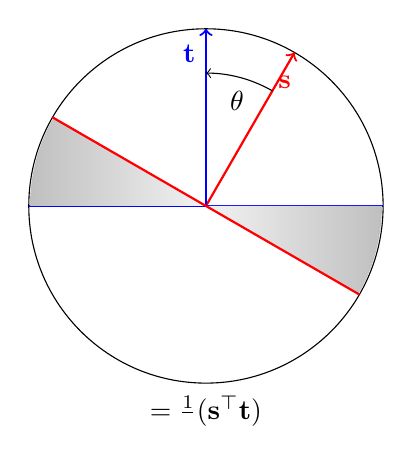
\begin{tikzpicture}[scale=1.5]

    % Circle
    \draw (0, 0) circle (1.5cm);

    % Vectors s (red at 60°) and t (blue at 90°)
    \draw[->,thick,red]  (0,0) -- (60:1.5cm) node[pos=0.7, above right] {\(\mathbf{s}\)};
    \draw[->,thick,blue] (0,0) -- (90:1.5cm) node[pos=0.75, above left] {\(\mathbf{t}\)};

    % Angle theta (between s & t)
    \draw[<-] (0,1.125) arc (90:60:1.125cm) node[pos=0.7, below left] {\(\theta\)};

    % Blue lines (perp. to t = 90°)
    \draw[thick,blue] (0,0) -- (-1.5,0);
    \draw[thick,blue] (0,0) -- ( 1.5,0);

    % Gray shading for overlap region
    \shade[left color=gray!50, right color=gray!10]
      (0,0) -- (-1.49,0) arc (180:150:1.5cm) -- cycle;
    \shade[left color=gray!10, right color=gray!50]
      (0,0) -- (1.49,0) arc (0:-30:1.5cm) -- cycle;

    % Red line(s) perp. to s (60°)
    \draw[thick,red]  (0,0) -- (150:1.5);
    \draw[thick,red]  (0,0) -- (330:1.5); % same as -30°

    % Overlap formula
    \node at (0,-1.75) {\( \AVGR = \frac{1}{\ND} (\mathbf{s}^\top \mathbf{t}) \)};

\end{tikzpicture}
\end{minipage}%
\hfill
%-------------------------------%
% Right image: 3D Overlap (conic sections + wedge)
%-------------------------------%
\begin{minipage}{0.48\linewidth}
\centering
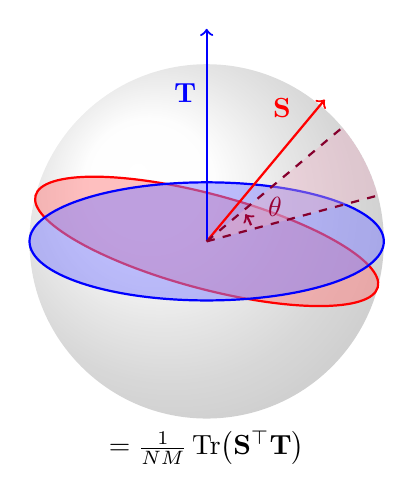
\begin{tikzpicture}[scale=1.5]

    % Light-gray "sphere"
    \shade[ball color=gray!5, opacity=0.3] (0,0) circle (1.5cm);

    % --- Red ellipse for S (unchanged) ---
    \begin{scope}
      \clip (0,0) circle (1.5cm);
      \fill[red!50, opacity=0.5]
        [rotate around={-15:(0,0)}, xscale=1.5, yscale=0.4]
        (0,0) circle (1.0);
    \end{scope}
    \draw[thick, red]
      [rotate around={-15:(0,0)}, xscale=1.5, yscale=0.4]
      (0,0) circle (1.0);

    % --- Blue ellipse for T (CHANGED) ---
    % Make it near-horizontal (rotate=0 or a small angle),
    % and bigger horizontally by increasing xscale significantly.
    \begin{scope}
      \clip (0,0) circle (1.5cm);
      \fill[blue!50, opacity=0.5]
        [rotate around={0:(0,0)},    % CHANGED: no tilt so near x-axis
         xscale=1.5, yscale=0.5]     % CHANGED: bigger horizontally
        (0,0) circle (1.0);
    \end{scope}
    \draw[thick, blue]
      [rotate around={0:(0,0)}, xscale=1.5, yscale=0.5]
      (0,0) circle (1.0);

    % Vectors S (red) & T (blue, vertical & longer)
    \draw[->,thick,red]  (0,0) -- (1.0,1.2)
      node[pos=0.8, above left]  {\(\mathbf{S}\)};
    \draw[->,thick,blue] (0,0) -- (0,1.8)
      node[pos=0.7, left] {\(\mathbf{T}\)};

    % Remove old "theta" arcs

    % -- Fill a wedge (solid angle) in purple --
    \begin{scope}
      \clip (0,0) circle (1.5cm);
      % Let’s pick a narrower wedge from ~15° to ~40°
      \fill[purple!30, opacity=0.4]
        (0,0)
         -- (15:1.5cm)
         arc [start angle=15, end angle=40, radius=1.5cm]
         -- cycle;
    \end{scope}

    % Dashed wedge boundaries
    \draw[thick, dashed, purple!70!black] (0,0) -- (15:1.5cm);
    \draw[thick, dashed, purple!70!black] (0,0) -- (40:1.5cm);

    % Single arc to label theta
    \draw[->, thick, purple!80!black]
      (20:0.4) arc[start angle=20, end angle=35, radius=0.4];
    \node[purple!80!black] at (27:0.65) {\(\theta\)};

    % Overlap formula
    \node at (0,-1.75) {\( \AVGR = \frac{1}{NM} \,\mathrm{Tr}\bigl(\mathbf{S}^\top \mathbf{T}\bigr) \)};

\end{tikzpicture}
\end{minipage}

% Main caption
\caption{Comparison of 2D and 3D representations of the vector and matrix Student--Teacher overlap \(R\).
\textbf{Left:} \(\AVGR = \tfrac{1}{\ND}\mathbf{s}^\top \mathbf{t}\).  Averaged over $\ND$ data samples (implicitly normalized to $1/m$).
\textbf{Right:} \(R = \tfrac{1}{NM}\,\mathrm{Tr}\bigl(\mathbf{S}^\top\mathbf{T}\bigr)\) with conic sections on the sphere (red \(\mathbf{S}\), blue \(\mathbf{T}\)), plus a purple wedge for the angle.  Averaged over matrix dimensions $N$ and $M$ (implicitly normalized over the data $1/\ND$).}
\label{fig:overlaps}
\end{figure}

%\caption{Comparison of 2D and 3D representations of matrix overlap $R$. (a) 2D visualization of vector overlap $R = \cos(\theta) $.
%  (b) 3D visualization of matrix overlap $R = \Trace{\frac{1}{N^2} \SMAT^\top \TMAT $ with solid angle $R$.}



%%\subsubsection{Derivation of the  ST error $(\EPSL(\AVGR))$ for the Linear Perceptron}
\paragraph{Derivation of the  ST error $(\EPSL(\AVGR))$ for the Linear Perceptron.}
%\nred{WARNING: there may be some mistakes here}
To derive \EQN~\ref{eqn:LinearPerceptronError},
define the data-dependent ST error (\EQN~\ref{eqn:DE_L}) in terms of an $\ell_2$ loss function
%\begin{align}
%\nonumber
%\Delta \mathbf{E}_{\ell_2}(\SVEC,\TVEC,\XI) = & \frac{1}{2} (\Ys - \Yt)^T(\Ys - \Yt) 
%   = 1 - (\YsVEC)^{\top}(\YtVEC) \\ 
%\label{eqn:deriveSTerror}
%   =&  1 - \eta(\XI),
%\end{align}
\red{THIS SECTION HAS SOME TYPOS}

\begin{align}
\nonumber
\DETOPSTLL= & \frac{1}{2} (\YsVEC - \YtVEC)^{\top} (\YsVEC - \YtVEC) \\
\nonumber
=& \frac{1}{2} \big[(\YsVEC)^{\top} \YsVEC - 2 (\YsVEC)^{\top} \YtVEC + (\YtVEC)^{\top} \YtVEC \big] \\
\nonumber
=& \ND - (\YsVEC)^{\top} (\YtVEC) \\
\label{eqn:deriveSTerror}
=& \ND- \ETA(\SVEC,\TVEC,\red{\NDXI}),
\end{align}
where we define $\ETA(\SVEC,\TVEC,\red{\NDXI}):=\mathbf{y}_{S}^{\top}\mathbf{y}_{T}$, called
the \emph{data-dependent \SelfOverlap}; we expand this below.
The expression $\ETA(\SVEC,\TVEC,\XI)$ is analogous to the ST overlap $R$, but before the data has been integrated out.
It is convenient to work directly with
the \SelfOverlap $\ETA(\SVEC,\TVEC,\XI)$ because it will appear later in \EQN~\ref{eqn:eta_mat_avg_def} (in Section~\ref{sxn:matgen}), 
when formulating the matrix-generalized overlap operator~$\OVERLAP$.

In defining $\ETA(\SVEC,\TVEC,\XI)$, we replace the labels $(\mathbf{y}_{S},\mathbf{y}_{T})$ with the Energy functions $E_{NN}$  that generate them, giving an expression in terms of the weights $(\SVEC,\TVEC)$ and the Gaussian data variables $(\XI)$. We will then integrate out the data variables, leaving an expression just in terms of the weights.  
Using the $E_{NN}$ Energy generating or output function (\EQN~\ref{eqn:dnn_energy}, \ref{eqn:S_ENN}, \ref{eqn:T_ENN}), we can replace the label vectors $\YtVEC,\YsVEC$ as
\begin{align}
\YsVEC=\SVEC^{\top}\XI,\;\;
\YtVEC=\TVEC^{\top}\XI  ,
\end{align}
which gives
\begin{align}
  \label{eqn:eta_vec_xi_def}
\ETA(\SVEC,\TVEC,\XI) =\red{\sum_{\mu=1}^{\ND}} (\SVEC^{\top}\XI)^{\top} (\TVEC^{\top}\XI) = \red{\sum_{\mu=1}^{\ND}}\XI^{\top}_{\red{\mu}}  (\SVEC^{\top} \TVEC )\XI_{\red{\mu}} 
\end{align}
\red{THIS SECTION HAS SOME TYPOS}
or, more simply, after integrating over the data, we have the \emph{data-independent \SelfOverlap}
\begin{align}
  \label{eqn:eta_vec_avg_def}
\ETA(\SVEC,\TVEC) = \langle\ETA(\SVEC,\TVEC,\XI)\rangle_{\AVGNDXI}=\SVEC^{\top} \TVEC 
\end{align}

We want to evaluate this as an \EffectivePotential $\EPSL(\AVGR)$ for the data-averaged ST test error, as in \EQN~\ref{eqn:STerror}.
To do this, we need to compute the average or \ExpectedValue over all $\ND$ possible input data vectors $\NDXI (i.e., $d\mu(\NDXI)=\mathcal{D}\NDXI P(\NDXI)$).
%
\red{BELOW IS WRONG NEEDS FIED}
\begin{align}
 \langle\DETOPSTLL\rangle_{\AVGNDXI}  
   = & \int d\mu(\NDXI)(1-\ETA(\XI)) \\ \nonumber
   = & \int d\mu(\NDXI)(1-\XI^{\top}\tfrac{1}{\ND}\SVEC^{\top}\TVEC\XI) \\ \label{eqn:XI_ST} 
   = & \int d\mu(\NDXI)-\int d\mu(\NDXI)\XI^{\top}\tfrac{1}{\ND}\SVEC^{\top}\TVEC\XI)  \\ \nonumber
   = & 1 - \int d\mu(\NDXI)\XI^{\top}\tfrac{1}{\ND}\SVEC^{\top}\TVEC\XI \\ \nonumber
   = & 1 - \int d\mu(\XI)\XI^{\top} \AVGR\XI \\ \nonumber
   = &1 - \AVGR\int d\mu(\XI)\XI^{\top}\XI,
\end{align}
where this holds because the elements of $\XI$ are i.i.d.
Since $d\mu(\NDXI)$ is a measure over a (multi-variate) Gaussian distribution,
The data vectors $\XI$ are normalized (See Section~\ref{app:st-gen-err-annealed-ham}) such that the second term on the R.H.S. is unity and we recover (i.e.,\EQN~\ref{eqn:epsl})
\begin{align}
\label{eqn:e0}
\EPSL(\AVGR)=\langle\DETOPSTLL\rangle_{\AVGNDXI} =  1 - \AVGR .
\end{align}


In traditional \STATMECH (e.g., \cite{SST92}), one is interested in how the \emph{\TotalModelGeneralizationError} $\TGE(\AVGR)$ depends on $\AVGR$.
With these simple error functions, \EQN~\ref{eqn:MGE} reduces to a function over $\AVGR$,
and the \AverageSTGeneralizationError $\STGE(\AVGR)$ is then obtained by averaging over the Students 
\begin{align}
\label{eqn:AVGSTGE_R}
\AVGSTGE(\AVGR)=\THRMAVG{\EPSL(\AVGR)}=
\THRMAVG{1-\langle\ETA(\SVEC,\TVEC,\XI)\rangle_{\AVGNDXI}}=
\THRMAVG{1-\ETA(\SVEC,\TVEC)}=
\THRMAVG{1-\SVEC^{\top}\TVEC}=
\THRMAVG{(1-\AVGR)}  ,
\end{align}
where $\THRMAVG{\cdots}$ is a \ThermalAverage over the \Student weight vector $\SVEC$.

The \ModelQuality for the ST \Perceptron, $\Q^{ST}$
is just the \AverageGeneralizationAccuracy, so we can write
\begin{align}
\label{eqn:QST_final}
\Q^{ST} := 1 - \AVGSTGE(\AVGR) 
       = \THRMAVG{1 - \EPSL(\AVGR)} 
       = \THRMAVG{\langle\ETA(\SVEC, \TVEC, \XI)\rangle_{\AVGNDXI}} 
       = \THRMAVG{\ETA(\SVEC, \TVEC)} 
       = \THRMAVG{\SVEC^{\top}\TVEC} 
       = \THRMAVG{\AVGR}.
\end{align}
\EQN~\ref{eqn:QST_final} is the starting point for deriving a \SEMIEMP theory for the \WW quality metrics (\ALPHA,\ALPHAHAT);
see Section~\ref{sxn:matgen_mlp3}.
To generalize this expression, we will start with the \SelfOverlap $\ETA(\SMAT,\TMAT,\XI)$ for a
\MultiLayerPerceptron (MLP3) in Section~\ref{sxn:matgen}.

Before doing this, however, we note that 
we can obtain this expression for $\STGE$ by defining the
\AnnealedHamiltonian $\HANHT(\AVGR)$, at high-Temperature, as in Section~\ref{sxn:mathP}, \EQN~\ref{eqn:Gan_highT_final}.
\nred{I H a fcn or avg R?}
Indeed, it is really $\HANHT(\AVGR)=\EPSL(\AVGR)$ that we must generalize to the matrix case, which we do (using a technique
similar to a Replica calculation, but still in the AA).
For more details, see Appendix~\ref{sxn:summary_sst92}.
(In particular, doing this allows us to define the normalization needed later for the \TRACELOG condition).
\michaeladdressed{MM TO DO: still to work on this par.}


\begin{table}[t]
  \raggedright
\hspace*{-1.5cm}% Adjust this value as needed
\renewcommand{\arraystretch}{1.25} % Increase line spacing in table
\begin{tabular}{|c|c|c|c|}
  \hline
  Quantity & Traditional \SMOG & \makecell{\LinearPerceptron \\ in Traditional \SMOG} & \makecell{Matrix Generalization \\ for \SETOL} \\ \hline

  Total (Idealized) Data Error 
    & $\DETOPXI$ (\ref{eqn:detox})
    & $\DETOPSTL$ (\ref{eqn:deriveSTerror}) 
    & $\DETOPNN$ (\ref{eqn:DE2}) \\ \hline

   Annealed Hamiltonian
    & $\HANHT=\EPSLw$ (\ref{eqn:epsl}) 
    & $\GANHTR=\EPSLSTx=1-\AVGR$ (\ref{eqn:epslR}) 
  & $\GANMATHT = N(\IM-\OVERLAP)$ (\ref{eqn:GANHTmatR}) \\

  (Data-Averaged Error) 
    & (AA, at high-T) 
    & (and at \LargeN) 
    & (only for a layer)  \\ \hline

    \SelfOverlap 
    & $\ETAw = 1-\EPSLw$~(\ref{eqn:def_eta})

    & $\ETA(\SVEC,\TVEC)=\SVEC^{\top}\TVEC$ (\ref{eqn:eta_vec_avg_def})
    & $\ETA(\SMAT,\TMAT)=\tfrac{1}{N}\SMAT^{\top}\TMAT$ (\ref{eqn:eta_mat_avg_def})  \\ \hline
    \hline

  \ModelQuality 
    & $\Q:=1-\AVGGE$ 
    & $\Q^{ST}:=1-\AVGGE^{ST}$ (\ref{eqn:model_qualities})
   & $\Q^{NN}:=1-\AVGGE^{NN}$  (\ref{eqn:model_qualities})\\ 

  in terms of \LayerQuality
    & 
    & 
   & $\Q^{NN}:=\prod_{L} \Q^{NN}_{L}$ \\ \hline
\end{tabular}
\caption{Summary of key quantities compared across traditional \SMOG models,  the \Student-\Teacher (ST) \LinearPerceptron--in the \AnnealedApproximation
(AA) and at high-Temperature (high-T) and at \LargeN in $\ND$, and the matrix-generalized forms as the starting point to frame \SETOL.
The total ST Error of Energy, $\DELBF$, represents the difference (squared) between the model and its labels for the ST model between
the \Student and \Teacher predictions.
The \AnnealedHamiltonian is the Energy function for this Error after it is averaged over the model for the training data
(an $\ND$-dimensional i.i.d. idealized Gaussian dataset,  $\NDXIn$).
In the AA, the \AnnealedHamiltonian is equal to the \EffectivePotential.  For the ST model,  this is one minus the average overlap, $\HANHT(R)=(1-\AVGR)$;
for the \SETOL, this is  the ($M$-dimensional) identity minus the overlap operator/matrix, $\HANHT(\OVERLAP)=N(\IM-\OVERLAP)$. 
The \SelfOverlap $\eta(\cdots)$ is used to describe the Accuracy (as opposed to the Error) for both the ST model and
its matrix-generalized form.
%Notice that $\eta(\XI)$, as defined,  has not yet been averaged over the model data $\XI^{N}$.
Finally, the different forms of the \Quality are defined.  Generally speaking, the \Quality $\Q$ is an approximation to some measure
of $1$ minus the \AverageGeneralizationError, $\Q:=1-\AVGGE$ (in the AA, at high-T, at \LargeN, and with whatever else
approximations are applied).
For the ST model, having just 1 layer, the \ModelQuality and the \LayerQuality are the same, and denoted $\Q^{ST}$.
For \SETOL, the \ModelQuality $\Q^{NN}$ is a product of individual \LayerQualities $\Q^{NN}_{L}$.
(Note that the  final \SETOL \LayerQuality $\Q$ is defined in terms of the \LayerQualitySquared $\QT$,
and the starting point for this is expressed with the \LayerQualitySquared Hamiltonian $\HBARE=\OLAPTOLAP$.
}
\label{table:quantities_general_vect_matrix}
\end{table}


\clearpage
